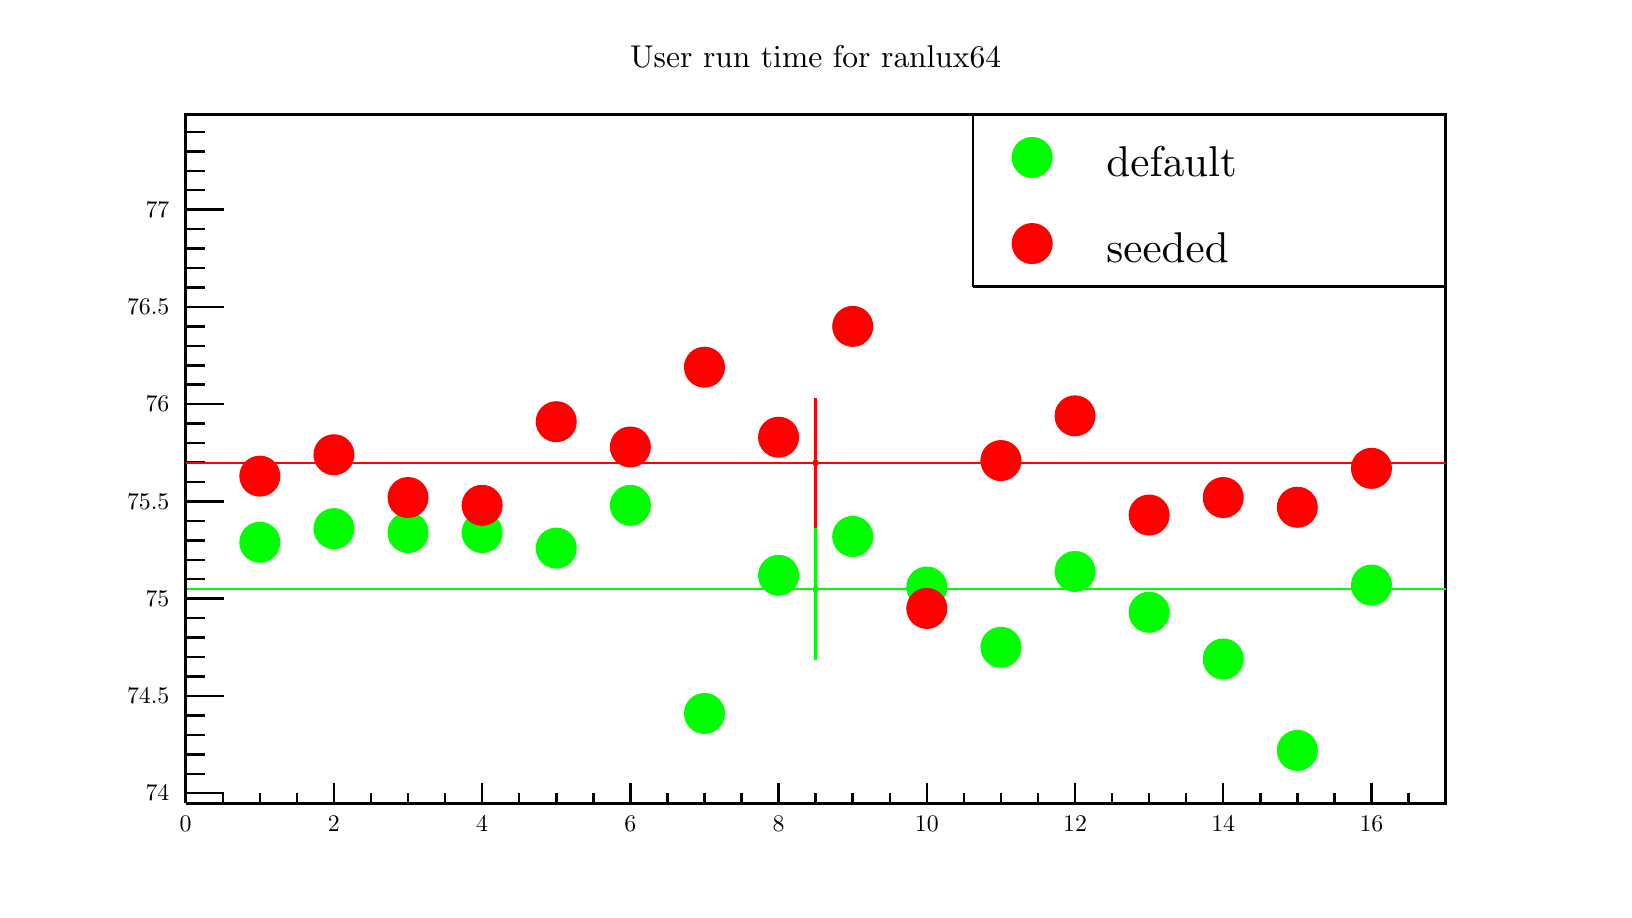
\begin{tikzpicture}
\pgfdeclareplotmark{cross} {
\pgfpathmoveto{\pgfpoint{-0.3\pgfplotmarksize}{\pgfplotmarksize}}
\pgfpathlineto{\pgfpoint{+0.3\pgfplotmarksize}{\pgfplotmarksize}}
\pgfpathlineto{\pgfpoint{+0.3\pgfplotmarksize}{0.3\pgfplotmarksize}}
\pgfpathlineto{\pgfpoint{+1\pgfplotmarksize}{0.3\pgfplotmarksize}}
\pgfpathlineto{\pgfpoint{+1\pgfplotmarksize}{-0.3\pgfplotmarksize}}
\pgfpathlineto{\pgfpoint{+0.3\pgfplotmarksize}{-0.3\pgfplotmarksize}}
\pgfpathlineto{\pgfpoint{+0.3\pgfplotmarksize}{-1.\pgfplotmarksize}}
\pgfpathlineto{\pgfpoint{-0.3\pgfplotmarksize}{-1.\pgfplotmarksize}}
\pgfpathlineto{\pgfpoint{-0.3\pgfplotmarksize}{-0.3\pgfplotmarksize}}
\pgfpathlineto{\pgfpoint{-1.\pgfplotmarksize}{-0.3\pgfplotmarksize}}
\pgfpathlineto{\pgfpoint{-1.\pgfplotmarksize}{0.3\pgfplotmarksize}}
\pgfpathlineto{\pgfpoint{-0.3\pgfplotmarksize}{0.3\pgfplotmarksize}}
\pgfpathclose
\pgfusepathqstroke
}
\pgfdeclareplotmark{cross*} {
\pgfpathmoveto{\pgfpoint{-0.3\pgfplotmarksize}{\pgfplotmarksize}}
\pgfpathlineto{\pgfpoint{+0.3\pgfplotmarksize}{\pgfplotmarksize}}
\pgfpathlineto{\pgfpoint{+0.3\pgfplotmarksize}{0.3\pgfplotmarksize}}
\pgfpathlineto{\pgfpoint{+1\pgfplotmarksize}{0.3\pgfplotmarksize}}
\pgfpathlineto{\pgfpoint{+1\pgfplotmarksize}{-0.3\pgfplotmarksize}}
\pgfpathlineto{\pgfpoint{+0.3\pgfplotmarksize}{-0.3\pgfplotmarksize}}
\pgfpathlineto{\pgfpoint{+0.3\pgfplotmarksize}{-1.\pgfplotmarksize}}
\pgfpathlineto{\pgfpoint{-0.3\pgfplotmarksize}{-1.\pgfplotmarksize}}
\pgfpathlineto{\pgfpoint{-0.3\pgfplotmarksize}{-0.3\pgfplotmarksize}}
\pgfpathlineto{\pgfpoint{-1.\pgfplotmarksize}{-0.3\pgfplotmarksize}}
\pgfpathlineto{\pgfpoint{-1.\pgfplotmarksize}{0.3\pgfplotmarksize}}
\pgfpathlineto{\pgfpoint{-0.3\pgfplotmarksize}{0.3\pgfplotmarksize}}
\pgfpathclose
\pgfusepathqfillstroke
}
\pgfdeclareplotmark{newstar} {
\pgfpathmoveto{\pgfqpoint{0pt}{\pgfplotmarksize}}
\pgfpathlineto{\pgfqpointpolar{44}{0.5\pgfplotmarksize}}
\pgfpathlineto{\pgfqpointpolar{18}{\pgfplotmarksize}}
\pgfpathlineto{\pgfqpointpolar{-20}{0.5\pgfplotmarksize}}
\pgfpathlineto{\pgfqpointpolar{-54}{\pgfplotmarksize}}
\pgfpathlineto{\pgfqpointpolar{-90}{0.5\pgfplotmarksize}}
\pgfpathlineto{\pgfqpointpolar{234}{\pgfplotmarksize}}
\pgfpathlineto{\pgfqpointpolar{198}{0.5\pgfplotmarksize}}
\pgfpathlineto{\pgfqpointpolar{162}{\pgfplotmarksize}}
\pgfpathlineto{\pgfqpointpolar{134}{0.5\pgfplotmarksize}}
\pgfpathclose
\pgfusepathqstroke
}
\pgfdeclareplotmark{newstar*} {
\pgfpathmoveto{\pgfqpoint{0pt}{\pgfplotmarksize}}
\pgfpathlineto{\pgfqpointpolar{44}{0.5\pgfplotmarksize}}
\pgfpathlineto{\pgfqpointpolar{18}{\pgfplotmarksize}}
\pgfpathlineto{\pgfqpointpolar{-20}{0.5\pgfplotmarksize}}
\pgfpathlineto{\pgfqpointpolar{-54}{\pgfplotmarksize}}
\pgfpathlineto{\pgfqpointpolar{-90}{0.5\pgfplotmarksize}}
\pgfpathlineto{\pgfqpointpolar{234}{\pgfplotmarksize}}
\pgfpathlineto{\pgfqpointpolar{198}{0.5\pgfplotmarksize}}
\pgfpathlineto{\pgfqpointpolar{162}{\pgfplotmarksize}}
\pgfpathlineto{\pgfqpointpolar{134}{0.5\pgfplotmarksize}}
\pgfpathclose
\pgfusepathqfillstroke
}
\definecolor{c}{rgb}{1,1,1};
\draw [color=c, fill=c] (0,0) rectangle (20,10.9387);
\draw [color=c, fill=c] (2,1.09387) rectangle (18,9.84481);
\definecolor{c}{rgb}{0,0,0};
\draw [c,line width=0.9] (2,1.09387) -- (2,9.84481) -- (18,9.84481) -- (18,1.09387) -- (2,1.09387);
\definecolor{c}{rgb}{1,1,1};
\draw [color=c, fill=c] (2,1.09387) rectangle (18,9.84481);
\definecolor{c}{rgb}{0,0,0};
\draw [c,line width=0.9] (2,1.09387) -- (2,9.84481) -- (18,9.84481) -- (18,1.09387) -- (2,1.09387);
\definecolor{c}{rgb}{0,1,0};
\draw [c,line width=0.9] (10,2.91908) -- (10,3.81426);
\draw [c,line width=0.9] (10,3.81426) -- (10,4.70943);
\draw [c,line width=0.9] (2,3.81426) -- (10,3.81426);
\draw [c,line width=0.9] (10,3.81426) -- (18,3.81426);
\foreach \P in {(10,3.81426)}{\draw[mark options={color=c,fill=c},mark size=2.402402pt,mark=*,mark size=1pt] plot coordinates {\P};}
\definecolor{c}{rgb}{0,0,0};
\draw [c,line width=0.9] (2,1.09387) -- (18,1.09387);
\draw [c,line width=0.9] (2,1.3564) -- (2,1.09387);
\draw [c,line width=0.9] (2.47059,1.22513) -- (2.47059,1.09387);
\draw [c,line width=0.9] (2.94118,1.22513) -- (2.94118,1.09387);
\draw [c,line width=0.9] (3.41176,1.22513) -- (3.41176,1.09387);
\draw [c,line width=0.9] (3.88235,1.3564) -- (3.88235,1.09387);
\draw [c,line width=0.9] (4.35294,1.22513) -- (4.35294,1.09387);
\draw [c,line width=0.9] (4.82353,1.22513) -- (4.82353,1.09387);
\draw [c,line width=0.9] (5.29412,1.22513) -- (5.29412,1.09387);
\draw [c,line width=0.9] (5.76471,1.3564) -- (5.76471,1.09387);
\draw [c,line width=0.9] (6.23529,1.22513) -- (6.23529,1.09387);
\draw [c,line width=0.9] (6.70588,1.22513) -- (6.70588,1.09387);
\draw [c,line width=0.9] (7.17647,1.22513) -- (7.17647,1.09387);
\draw [c,line width=0.9] (7.64706,1.3564) -- (7.64706,1.09387);
\draw [c,line width=0.9] (8.11765,1.22513) -- (8.11765,1.09387);
\draw [c,line width=0.9] (8.58823,1.22513) -- (8.58823,1.09387);
\draw [c,line width=0.9] (9.05882,1.22513) -- (9.05882,1.09387);
\draw [c,line width=0.9] (9.52941,1.3564) -- (9.52941,1.09387);
\draw [c,line width=0.9] (10,1.22513) -- (10,1.09387);
\draw [c,line width=0.9] (10.4706,1.22513) -- (10.4706,1.09387);
\draw [c,line width=0.9] (10.9412,1.22513) -- (10.9412,1.09387);
\draw [c,line width=0.9] (11.4118,1.3564) -- (11.4118,1.09387);
\draw [c,line width=0.9] (11.8824,1.22513) -- (11.8824,1.09387);
\draw [c,line width=0.9] (12.3529,1.22513) -- (12.3529,1.09387);
\draw [c,line width=0.9] (12.8235,1.22513) -- (12.8235,1.09387);
\draw [c,line width=0.9] (13.2941,1.3564) -- (13.2941,1.09387);
\draw [c,line width=0.9] (13.7647,1.22513) -- (13.7647,1.09387);
\draw [c,line width=0.9] (14.2353,1.22513) -- (14.2353,1.09387);
\draw [c,line width=0.9] (14.7059,1.22513) -- (14.7059,1.09387);
\draw [c,line width=0.9] (15.1765,1.3564) -- (15.1765,1.09387);
\draw [c,line width=0.9] (15.6471,1.22513) -- (15.6471,1.09387);
\draw [c,line width=0.9] (16.1176,1.22513) -- (16.1176,1.09387);
\draw [c,line width=0.9] (16.5882,1.22513) -- (16.5882,1.09387);
\draw [c,line width=0.9] (17.0588,1.3564) -- (17.0588,1.09387);
\draw [c,line width=0.9] (17.0588,1.3564) -- (17.0588,1.09387);
\draw [c,line width=0.9] (17.5294,1.22513) -- (17.5294,1.09387);
\draw [c,line width=0.9] (18,1.22513) -- (18,1.09387);
\draw [anchor=base] (2,0.732891) node[scale=0.861703, color=c, rotate=0]{0};
\draw [anchor=base] (3.88235,0.732891) node[scale=0.861703, color=c, rotate=0]{2};
\draw [anchor=base] (5.76471,0.732891) node[scale=0.861703, color=c, rotate=0]{4};
\draw [anchor=base] (7.64706,0.732891) node[scale=0.861703, color=c, rotate=0]{6};
\draw [anchor=base] (9.52941,0.732891) node[scale=0.861703, color=c, rotate=0]{8};
\draw [anchor=base] (11.4118,0.732891) node[scale=0.861703, color=c, rotate=0]{10};
\draw [anchor=base] (13.2941,0.732891) node[scale=0.861703, color=c, rotate=0]{12};
\draw [anchor=base] (15.1765,0.732891) node[scale=0.861703, color=c, rotate=0]{14};
\draw [anchor=base] (17.0588,0.732891) node[scale=0.861703, color=c, rotate=0]{16};
\draw [c,line width=0.9] (2,1.09387) -- (2,9.84481);
\draw [c,line width=0.9] (2.48,1.22356) -- (2,1.22356);
\draw [c,line width=0.9] (2.24,1.47058) -- (2,1.47058);
\draw [c,line width=0.9] (2.24,1.71761) -- (2,1.71761);
\draw [c,line width=0.9] (2.24,1.96464) -- (2,1.96464);
\draw [c,line width=0.9] (2.24,2.21167) -- (2,2.21167);
\draw [c,line width=0.9] (2.48,2.45869) -- (2,2.45869);
\draw [c,line width=0.9] (2.24,2.70572) -- (2,2.70572);
\draw [c,line width=0.9] (2.24,2.95275) -- (2,2.95275);
\draw [c,line width=0.9] (2.24,3.19977) -- (2,3.19977);
\draw [c,line width=0.9] (2.24,3.4468) -- (2,3.4468);
\draw [c,line width=0.9] (2.48,3.69383) -- (2,3.69383);
\draw [c,line width=0.9] (2.24,3.94086) -- (2,3.94086);
\draw [c,line width=0.9] (2.24,4.18788) -- (2,4.18788);
\draw [c,line width=0.9] (2.24,4.43491) -- (2,4.43491);
\draw [c,line width=0.9] (2.24,4.68194) -- (2,4.68194);
\draw [c,line width=0.9] (2.48,4.92896) -- (2,4.92896);
\draw [c,line width=0.9] (2.24,5.17599) -- (2,5.17599);
\draw [c,line width=0.9] (2.24,5.42302) -- (2,5.42302);
\draw [c,line width=0.9] (2.24,5.67005) -- (2,5.67005);
\draw [c,line width=0.9] (2.24,5.91707) -- (2,5.91707);
\draw [c,line width=0.9] (2.48,6.1641) -- (2,6.1641);
\draw [c,line width=0.9] (2.24,6.41113) -- (2,6.41113);
\draw [c,line width=0.9] (2.24,6.65815) -- (2,6.65815);
\draw [c,line width=0.9] (2.24,6.90518) -- (2,6.90518);
\draw [c,line width=0.9] (2.24,7.15221) -- (2,7.15221);
\draw [c,line width=0.9] (2.48,7.39924) -- (2,7.39924);
\draw [c,line width=0.9] (2.24,7.64626) -- (2,7.64626);
\draw [c,line width=0.9] (2.24,7.89329) -- (2,7.89329);
\draw [c,line width=0.9] (2.24,8.14032) -- (2,8.14032);
\draw [c,line width=0.9] (2.24,8.38735) -- (2,8.38735);
\draw [c,line width=0.9] (2.48,8.63437) -- (2,8.63437);
\draw [c,line width=0.9] (2.48,1.22356) -- (2,1.22356);
\draw [c,line width=0.9] (2.48,8.63437) -- (2,8.63437);
\draw [c,line width=0.9] (2.24,8.8814) -- (2,8.8814);
\draw [c,line width=0.9] (2.24,9.12843) -- (2,9.12843);
\draw [c,line width=0.9] (2.24,9.37545) -- (2,9.37545);
\draw [c,line width=0.9] (2.24,9.62248) -- (2,9.62248);
\draw [anchor= east] (1.9,1.22356) node[scale=0.861703, color=c, rotate=0]{74};
\draw [anchor= east] (1.9,2.45869) node[scale=0.861703, color=c, rotate=0]{74.5};
\draw [anchor= east] (1.9,3.69383) node[scale=0.861703, color=c, rotate=0]{75};
\draw [anchor= east] (1.9,4.92896) node[scale=0.861703, color=c, rotate=0]{75.5};
\draw [anchor= east] (1.9,6.1641) node[scale=0.861703, color=c, rotate=0]{76};
\draw [anchor= east] (1.9,7.39924) node[scale=0.861703, color=c, rotate=0]{76.5};
\draw [anchor= east] (1.9,8.63437) node[scale=0.861703, color=c, rotate=0]{77};
\definecolor{c}{rgb}{1,0,0};
\draw [c,line width=0.9] (10,4.59562) -- (10,5.41839);
\draw [c,line width=0.9] (10,5.41839) -- (10,6.24117);
\draw [c,line width=0.9] (2,5.41839) -- (10,5.41839);
\draw [c,line width=0.9] (10,5.41839) -- (18,5.41839);
\foreach \P in {(10,5.41839)}{\draw[mark options={color=c,fill=c},mark size=2.402402pt,mark=*,mark size=1pt] plot coordinates {\P};}
\definecolor{c}{rgb}{0,1,0};
\foreach \P in {(2.94118,4.41021), (3.88235,4.58313), (4.82353,4.53372), (5.76471,4.53372), (6.70588,4.3361), (7.64706,4.87956), (8.58823,2.23637), (9.52941,3.99026), (10.4706,4.48432), (11.4118,3.84204), (12.3529,3.07626), (13.2941,4.03967),
 (14.2353,3.52091), (15.1765,2.92804), (16.1176,1.76702), (17.0588,3.86675)}{\draw[mark options={color=c,fill=c},mark size=7.207207pt,mark=*] plot coordinates {\P};}
\definecolor{c}{rgb}{1,0,0};
\foreach \P in {(2.94118,5.2501), (3.88235,5.52183), (4.82353,4.97837), (5.76471,4.87956), (6.70588,5.94178), (7.64706,5.62064), (8.58823,6.63345), (9.52941,5.74415), (10.4706,7.15221), (11.4118,3.57031), (12.3529,5.44772), (13.2941,6.01588),
 (14.2353,4.75605), (15.1765,4.97837), (16.1176,4.85486), (17.0588,5.34891)}{\draw[mark options={color=c,fill=c},mark size=7.207207pt,mark=*] plot coordinates {\P};}
\definecolor{c}{rgb}{1,1,1};
\draw [color=c, fill=c] (12,7.65707) rectangle (18,9.84481);
\definecolor{c}{rgb}{0,0,0};
\draw [c,line width=0.9] (12,7.65707) -- (18,7.65707);
\draw [c,line width=0.9] (18,7.65707) -- (18,9.84481);
\draw [c,line width=0.9] (18,9.84481) -- (12,9.84481);
\draw [c,line width=0.9] (12,9.84481) -- (12,7.65707);
\draw [anchor=base west] (13.5,9.05175) node[scale=1.55662, color=c, rotate=0]{default};
\definecolor{c}{rgb}{1,1,1};
\draw [c] (12.225,8.91502) -- (13.275,8.91502) -- (13.275,9.68073) -- (12.225,9.68073);
\draw [c,line width=0.9] (12.225,9.29787) -- (13.275,9.29787);
\definecolor{c}{rgb}{0,1,0};
\foreach \P in {(12.75,9.29787)}{\draw[mark options={color=c,fill=c},mark size=7.207207pt,mark=*] plot coordinates {\P};}
\definecolor{c}{rgb}{0,0,0};
\draw [anchor=base west] (13.5,7.95788) node[scale=1.55662, color=c, rotate=0]{seeded};
\definecolor{c}{rgb}{1,1,1};
\draw [c] (12.225,7.82115) -- (13.275,7.82115) -- (13.275,8.58686) -- (12.225,8.58686);
\draw [c,line width=0.9] (12.225,8.204) -- (13.275,8.204);
\definecolor{c}{rgb}{1,0,0};
\foreach \P in {(12.75,8.204)}{\draw[mark options={color=c,fill=c},mark size=7.207207pt,mark=*] plot coordinates {\P};}
\definecolor{c}{rgb}{0,0,0};
\draw (10,10.5832) node[scale=1.13967, color=c, rotate=0]{User run time for ranlux64};
\end{tikzpicture}
